% !TeX program = xelatex
% !TeX root = ./main.tex
\documentclass[lang=cn,chinesefont=nofont,a4paper,newtx]{elegantpaper}

\setCJKmainfont[AutoFakeBold=2,AutoFakeSlant=.2]{STSong}
\setCJKmonofont{STSong}

\title{Hadamard Rotation 与 Lloyd-Max Codebook 在 TinyLlama 低比特量化中的实验报告}
\author{Carrey Liu}
\institute{Zhejiang University}

\version{0.1}
\date{\zhdate{2026/5/9}}

\addbibresource[location=local]{reference.bib}

\setlength{\floatsep}{6pt plus 2pt minus 2pt}
\setlength{\textfloatsep}{8pt plus 2pt minus 2pt}
\setlength{\intextsep}{6pt plus 2pt minus 2pt}
\setlength{\abovecaptionskip}{3pt}
\setlength{\belowcaptionskip}{0pt}
\setlength{\tabcolsep}{4pt}
\renewcommand{\arraystretch}{0.95}
\captionsetup{font=small,skip=3pt}
\renewcommand{\topfraction}{0.9}
\renewcommand{\bottomfraction}{0.8}
\renewcommand{\textfraction}{0.07}
\renewcommand{\floatpagefraction}{0.8}

\begin{document}

\maketitle

\begin{abstract}
本文记录 Rotation Quant 实验的设计、结果与结论。
\keywords{大语言模型量化，Hadamard rotation，Lloyd-Max，QuaRot，KV cache，QJL}
\end{abstract}

\section{综述}

\subsection{实验综述}

大语言模型的推理成本主要来自两类资源压力：一是权重、激活和 KV cache 的存储与访存开销，二是矩阵乘法与 attention 计算中的带宽和算力需求。低比特量化试图用更少的 bit 表示模型中的权重、激活或缓存张量，从而为降低部署成本提供可能。然而，对于后训练量化而言，数值分布中的 outlier、不同模块之间的误差传播，以及 attention score 对 key 内积误差的敏感性，都会使简单的 uniform absmax / round-to-nearest 量化在 4 bit 甚至 3 bit 下迅速失效。

本报告记录的 Rotation Quant 实验不直接研究真实硬件吞吐。实验的目标是先在可控的小模型上验证数值质量和低比特位宽边界：如果某种旋转域量化方法能够在 fake quant 环境中把可用位宽从 4 bit 推进到 3 bit，并且保持可接受的 tensor error、layer output error、attention score error 与 PPL，那么它可以作为后续 bit packing、codebook-aware MAC、LUT-based dequant 或专用 low-bit kernel 的算法依据。

这一阶段的实验围绕 TinyLlama 展开，并分为 A、B、C 三条线。A 线是 weight-only 实验，主要判断 Hadamard rotation 与 Lloyd-Max codebook 是否能使权重量化从 W4 推进到 W3。B 线是 W/A fake quantization，重点放在 FFN 模块中，验证旋转域的 `W3A4' 或 `W4A3' 是否能接近甚至优于 uniform `W4A4'。C 线面向 Attention 与 KV cache，先验证 post-RoPE key/query 的 head-wise rotation 是否保持 attention score，再评估 Hadamard-LM KV cache quantization、QJL residual correction，以及结构适配之后的完整 Attention 层数值质量。

这三条线构成递进关系。A 线探究权重本身是否适合 Hadamard + Lloyd-Max；B 线探究权重和激活共同量化后，局部 Linear 与完整 FFN 的非线性结构是否会放大量化误差。

\subsection{实验目的}

本实验的总目标是在 TinyLlama 上系统评估 Hadamard rotation、Lloyd-Max non-uniform codebook 与 QJL residual estimator 对低比特 W/A/KV 量化的作用。实验将统一记录 tensor-level、layer-level 与 model-level 指标，并把理论 bit label、scale / norm metadata 与 compute interpretation 分开讨论。

具体目标包括以下五点。第一，A 线判断 \texttt{Hadamard-LM W3} 在权重量化中是否具备可用性，并与 \texttt{MXFP4 W4}、\texttt{Hadamard-LM W4} 等强 4-bit baseline 比较。第二，B 线判断 \texttt{Rot-LM W3A4} 与 \texttt{Rot-LM W4A3} 在 FFN W/A fake quant 中是否仍能保持可接受的数值质量，并观察 FFN 中 gate/up/down 结构和 SiLU 非线性是否会放大误差。第三，C 线判断 \texttt{Hadamard-LM K3V4} 是否能保持 attention score、softmax KL、top-k overlap 与 attention output。第四，验证 QJL residual 是否能在 base key reconstruction 之后进一步修正 inner product bias。第五，比较 MXFP4、Lloyd-Max、不同 rotation backend 与 rotation block size 对最终 PPL 和局部误差的影响。

值得指出的是，本实验明确区分数值可行性与系统效率。Uniform absmax / RTN 结果较容易映射到 integer-like GEMM；Lloyd-Max 使用非均匀 centroid，需要 codebook lookup 或 dequant-aware 计算支持；QJL 使用 sign sketch 和 inner-product estimator，需要专门的 attention kernel。因而，本报告在第一阶段只给出数值质量、位宽边界和算法依据，不对真实吞吐、访存效率或端到端加速下结论。

\subsection{实验理论基础}

\subsubsection{Hadamard rotation 与 outlier smoothing}

QuaRot 的核心思想是利用正交旋转的计算不变性，将 LLM 中难以量化的 hidden state、FFN activation、attention activation 与 KV cache 转换到 outlier 更弱、动态范围更均匀的空间中，再进行低比特量化\cite{quarot2024}。设 $H$ 为正交 Hadamard 矩阵，若不考虑量化误差，则线性层可写为
\begin{equation}
  xW = (xH)(H^{T}W).
\end{equation}
由于 $H^{T}H=I$，该变换不改变原始线性计算；但在量化前，$xH$ 与 $H^{T}W$ 的坐标分布可能比原空间更平滑，从而降低单个 outlier 对 absmax scale 的支配作用。

这一性质是本实验使用 Hadamard rotation 的基础。A 线将 rotation 作用在权重上，观察 weight-only quantization 的位宽边界；B 线将相同思想用于 W/A fake quant，验证 activation outlier 被削弱后，低比特 activation 是否仍能保持 layer output；C 线则在 attention score 域中使用 head-wise H64 rotation，以保持 query-key 内积结构。

\subsubsection{Gaussian-like rotated weight 与 Lloyd-Max codebook}

Hadamard rotation 还为非均匀量化提供了分布条件。PolarQuant 指出，经过随机或结构化旋转后，高维权重向量的坐标分布更接近适合 Gaussian scalar quantizer 的形式，因此可以用针对 Gaussian 分布优化的 Lloyd-Max centroid 来降低量化失真\cite{polarquant2026}。与 uniform absmax quantization 不同，Lloyd-Max 不要求所有 code point 等间隔，而是根据目标分布的概率密度分配 centroid，使高概率区域获得更细的表示。

本实验中的 \texttt{hadamard\_lm} 与 \texttt{rot\_lm} 都属于 fake quant：张量先映射到旋转域，再按 block RMS 或 per-head RMS 归一化，随后用 Gaussian Lloyd-Max codebook 量化，最后以 centroid value 的形式反量化回浮点参与后续计算。

\subsubsection{W/A fake quant 的计算不变性}

B 线沿用 QuaRot 的计算不变性，但实验范围定在 local Linear、完整 FFN 和 FFN-only PPL。对于 PyTorch 中 shape 为 $[\text{out\_features}, \text{in\_features}]$ 的 Linear 权重，本实验沿最后一维应用 block-wise Hadamard。局部 fake quant 形式为
\begin{equation}
  \hat{y}
  =
  Q_A(xH)\,Q_W\!\bigl(H^{T}W\bigr){}^{T},
\end{equation}
其中 $Q_A$ 和 $Q_W$ 分别表示 activation 与 weight 的 fake quantizer。若 $Q_A$ 和 $Q_W$ 为 identity，该式与原始线性层等价；引入量化后，实验比较 Direct-Absmax、Rot-Absmax 与 Rot-LM 的输出误差。

\subsubsection{Attention/KV cache 的 inner product preservation}

Attention 中 Key 的核心评价目标不是 reconstruction MSE，而是 inner product preservation。对于 query $q$ 和 key $k$，attention score 直接由 $q^{T}k/\sqrt{d_h}$ 决定；score 的 bias 和 variance 会进一步影响 softmax 分布、top-k attention pattern 与 value aggregation。因此 C 线优先记录 inner product error、score relative MSE、softmax KL 和 top-k overlap，再观察 K reconstruction MSE。

在 LLaMA-like attention 中，query 和 key 会先经过 RoPE。QuaRot 的 KV cache 思路可理解为 post-RoPE caching：先得到真实的 $Q_{\mathrm{rope}}$ 和 $K_{\mathrm{rope}}$，再对每个 head 的 64 维向量施加相同的正交旋转\cite{quarot2024}：
\begin{equation}
  Q_H = Q_{\mathrm{rope}}H_{64}, \qquad
  K_H = K_{\mathrm{rope}}H_{64}.
\end{equation}
未量化时，由于 $H_{64}$ 正交，有
\begin{equation}
  Q_{\mathrm{rope}}K_{\mathrm{rope}}^{T}
  =
  Q_H K_H^{T}.
\end{equation}
因此 key cache 可以存储 rotated and quantized $K_H$；decode 或 prefill 中的当前 query 在 RoPE 后在线旋转为 $Q_H$，再与 dequantized rotated key cache 计算 score。

Value 不经过 RoPE，但它决定 attention output。对 Attention 层进行结构适配时，Value 可保留在旋转域中参与加权求和，并将相应的正交变换吸收到输出投影权重中，而不必先把 Value 反旋回原域再接原始输出投影。设 $P$ 为 attention probability，由于 $P$ 只在 sequence 维加权，不作用于 feature/head 维，
\begin{equation}
  P(VH_{64}) = (PV)H_{64}.
\end{equation}
因此可以令
\begin{equation}
  O_H = P\,Q(VH_{64}), \qquad
  W_{o,\mathrm{abs}} = W_o H_{64,\mathrm{blockdiag}},
\end{equation}
并用 $O_H W_{o,\mathrm{abs}}^{T}$ 近似原始 attention output projection。该适配方式使 Value 的旋转域量化与 Attention 的原有线性结构保持一致。

\subsubsection{QJL residual 与 residual inner-product correction}

TurboQuant 指出，仅优化 MSE 的量化器可能在 inner product estimation 上引入 bias，因此可采用 two-stage 策略：先用 base quantizer 进行主要重构，再对 residual 使用 1-bit Quantized Johnson-Lindenstrauss transform 进行内积修正\cite{turboquant2025}。QJL 方法将 key 或 residual 经过 Gaussian JL projection 后取 sign bit，并用非对称 estimator 估计 query 与 quantized vector 的 inner product\cite{qjl}。

本实验中的 C3 沿用这一思想，但目标更窄：先用 Hadamard-LM 得到 key 的 base reconstruction，再对 residual 做 Gaussian-QJL sign sketch，判断修正项是否降低 attention score MSE 和 softmax KL。

\subsubsection{ISSCC slides 中的系统背景}

RotationQuant ISSCC slides 提供了本实验的系统背景：旋转域量化不仅是数值技巧，也可能成为未来低比特存储路径、codebook-aware compute 和专用 attention kernel 的算法基础\cite{rotationquant2026isscc}。不过，本实验仍严格限制在 PyTorch fake quant 与数值验证层面。也就是说，即使某个方法在 PPL 上接近 FP16，也只能说明该算法组合具有进一步工程化的潜力，不能直接说明它已经带来真实吞吐提升。

\subsection{实验环境}

本实验统一使用 TinyLlama 作为实验模型，checkpoint 为 TinyLlama-1.1B intermediate step 1431k-3T；完整 Hugging Face 名称与本地模型路径已记录在实验文档和每次正式运行的 metadata 中。该模型为 LLaMA-like 架构，共 22 层，hidden size 为 2048，FFN intermediate size 为 5632；attention 使用 32 个 query heads、4 个 KV heads，head dimension 为 64。A/B 线默认使用 block size 128，并补充比较 32/64/128 三种 rotation block size；C 线在 KV cache 上比较 head-wise H64 与 head-internal H32。

数据集采用 WikiText2 raw test split。正式 PPL 评估策略是：使用 512 个样本、2048 token evaluation window 与 2048 token stride。实验在 Apple Silicon 上使用 PyTorch MPS 后端运行。实验代码运行在 \texttt{rotationquant} conda 环境中，主要包版本由各 run 的 \texttt{run\_metadata.json} 记录：Python 3.11.14，PyTorch 2.11.0，Transformers 5.8.0，Datasets 4.8.5，NumPy 2.4.3，Pandas 3.0.2，TQDM 4.67.3。

\section{实验结果}

\subsection{A 线：Weight-only 量化}

A 线实验回答的问题是：在 TinyLlama 的 weight-only 量化中，Hadamard rotation 与 Lloyd-Max codebook 是否能降低权重量化误差，并使 W3 成为可运行的位宽候选。实验比较 Direct Absmax、MXFP4、Hadamard Absmax、Hadamard-MXFP4、Hadamard LM，并补充 randomized Hadamard 与 dense random orthogonal 的旋转消融。评价指标包括权重 tensor reconstruction 质量和 model-level PPL。

表~\ref{tab:stage-a-tensor} 给出 154 个目标 Linear 权重上的 tensor reconstruction 汇总。MXFP4 W4 与 Hadamard Absmax W4 均显著降低 uniform quantization 的误差；在旋转域中使用 Lloyd-Max codebook 后，W4 与 W3 的 relative MSE 进一步下降。Hadamard-MXFP4 的 tensor MSE 低于未旋转 MXFP4，但仍高于 Hadamard LM W4。图~\ref{fig:stage-a-tensor-mse} 进一步显示，Lloyd-Max 在旋转域中具有更稳定的 reconstruction 优势。

\begin{table}[!htbp]
  \centering
  \caption{A 线权重 tensor reconstruction 汇总}
  \label{tab:stage-a-tensor}
  \begin{tabular}{lrrrr}
    \toprule
    Method & Bits & Relative MSE & Cosine & SQNR dB \\
    \midrule
    Direct Absmax & 4 & 0.0157 & 0.9925 & 18.1069 \\
    Direct Absmax & 3 & 0.0836 & 0.9613 & 10.8066 \\
    MXFP4 & 4 & 0.0141 & 0.9957 & 18.5087 \\
    Hadamard Absmax & 4 & 0.0138 & 0.9944 & 18.6095 \\
    Hadamard Absmax & 3 & 0.0751 & 0.9658 & 11.2464 \\
    Hadamard-MXFP4 & 4 & 0.0132 & 0.9946 & 18.7799 \\
    Hadamard LM & 4 & 0.0094 & 0.9966 & 20.2861 \\
    Hadamard LM & 3 & 0.0341 & 0.9841 & 14.6759 \\
    Hadamard LM & 2 & 0.1162 & 0.9413 & 9.3474 \\
    Rand-Hadamard LM & 4 & 0.0093 & 0.9966 & 20.3098 \\
    Rand-Hadamard LM & 3 & 0.0339 & 0.9841 & 14.6975 \\
    Rand-Ortho LM & 4 & 0.0093 & 0.9966 & 20.3001 \\
    Rand-Ortho LM & 3 & 0.0340 & 0.9841 & 14.6871 \\
    \bottomrule
  \end{tabular}
\end{table}

\begin{figure}[!htbp]
  \centering
  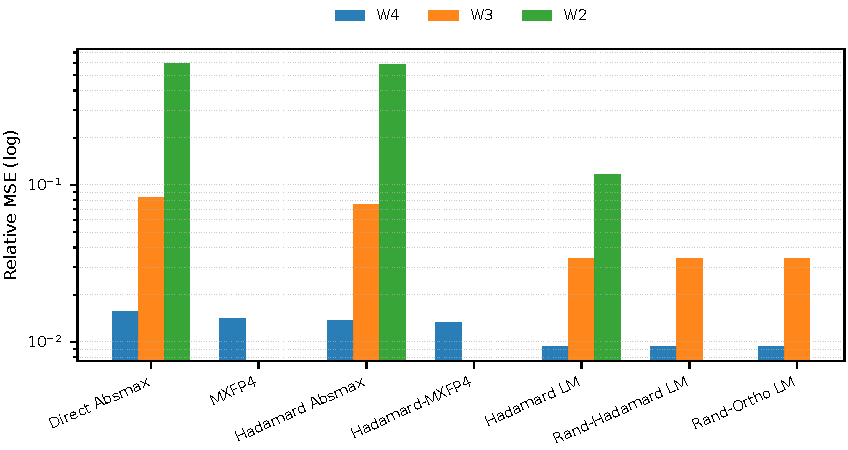
\includegraphics[width=0.82\linewidth]{image/stage_a_tensor_mse.pdf}
  \caption{A 线权重 relative MSE 对比}
  \label{fig:stage-a-tensor-mse}
\end{figure}

图~\ref{fig:stage-a-ppl} 给出 model-level PPL。FP16 的 PPL 为 8.05；Direct Absmax W4、MXFP4 W4、Hadamard Absmax W4 与 Hadamard LM W4 分别为 8.88、8.64、9.08 和 8.63。Hadamard-MXFP4 W4 的 PPL 为 8.95，未优于未旋转 MXFP4。Hadamard LM W3 与 randomized Hadamard LM W3 的 PPL 分别为 12.99 和 12.40，明显高于强 W4 baseline，但仍远低于 W2 失败组。Rotation backend 方面，randomized Hadamard 与普通 Hadamard 接近，dense random orthogonal 没有显示出稳定优势。

\begin{figure}[!htbp]
  \centering
  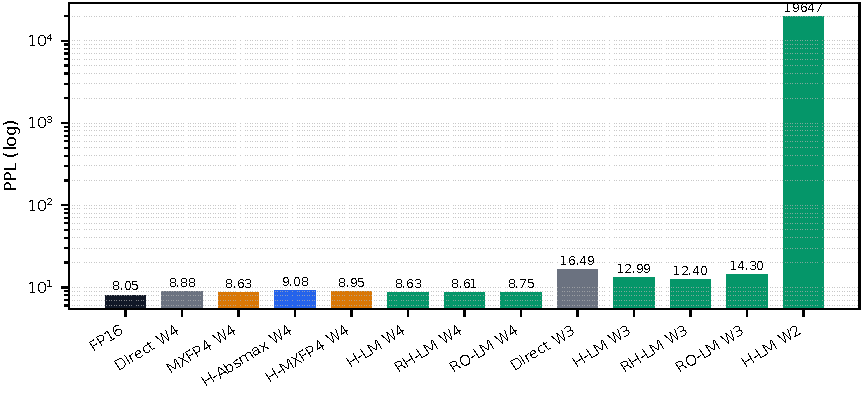
\includegraphics[width=0.88\linewidth]{image/stage_a_ppl.pdf}
  \caption{A 线 model-level PPL 对比；纵轴使用对数坐标}
  \label{fig:stage-a-ppl}
\end{figure}

综上，A 线得到三点发现。第一，MXFP4 W4 是强 baseline，PPL 接近 Hadamard LM W4。第二，Hadamard LM 在 tensor reconstruction 上最稳定，W4 的 model-level PPL 也最接近 FP16。第三，W3 具备可运行性，但相对 W4 baseline 仍存在明显 PPL gap；W2 暂时只能作为失败边界。

\subsection{B 线：FFN W/A Fake Quantization}

B 线实验回答的问题是：在 FFN 的 W/A fake quant 中，旋转域 Lloyd-Max 是否能使 W/A 位宽从 W4A4 推进到 W3A4 或 W4A3。实验按 activation tensor、local Linear/FFN output 和 FFN-only model-level PPL 三个层次展开，用于观察低一档 weight bit 或 activation bit 是否仍能保持数值质量。

实验比较 Direct-Absmax、MXFP4、Rot-Absmax、Rot-MXFP4 和 Rot-LM。Activation tensor-level 实验覆盖 A4/A3；local Linear/FFN 实验重点比较 W4A4 与 W3A4；FFN-only PPL 实验比较 FP16、FFN MXFP4 W4A4、FFN Rot-MXFP4 W4A4，以及 FFN Rot-LM 的 W4A4、W3A4 和 W4A3。

图~\ref{fig:stage-b-activation-mse} 给出关键 activation site 上的 relative MSE 对比。Rot-LM A4 在所有 site 上误差最低；Rot-MXFP4 A4 明显优于未旋转 MXFP4 A4。Rot-LM A3 的误差低于 Direct-Absmax A4，但高于 MXFP4 A4 与 Rot-MXFP4 A4，说明 activation 降至 3 bit 仍具备数值空间，但不能简单等同于强 4-bit baseline。

\begin{figure}[!htbp]
  \centering
  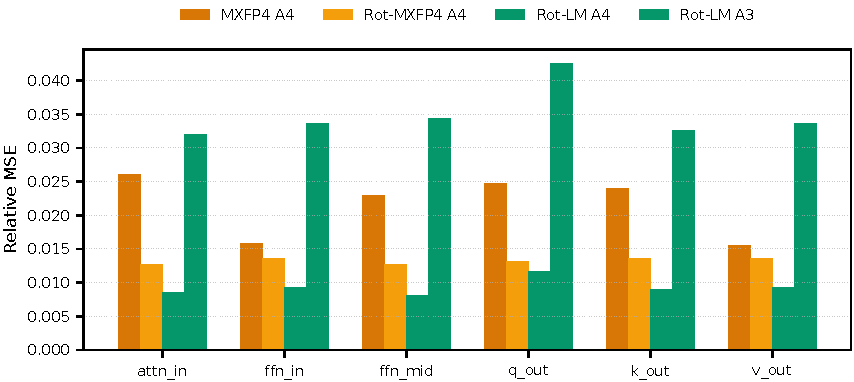
\includegraphics[width=0.86\linewidth]{image/stage_b_activation_mse.pdf}
  \caption{B 线 activation relative MSE 对比}
  \label{fig:stage-b-activation-mse}
\end{figure}

表~\ref{tab:stage-b-local} 汇总 local Linear 与完整 FFN output error。MXFP4 W4A4 已是较强 baseline；Rot-MXFP4 进一步降低 local error，但仍弱于 Rot-LM W4A4。Rot-LM W3A4 的误差高于 Rot-LM W4A4，但在 FFN local output 上仍处于可接受区间。

\begin{table}[!htbp]
  \centering
  \caption{B 线 local Linear/FFN output error 汇总}
  \label{tab:stage-b-local}
  \footnotesize
  \begin{tabular}{lllrrr}
    \toprule
    Scope & Method & Bits & Relative MSE & Cosine & SQNR dB \\
    \midrule
    Linear & MXFP4 & W4A4 & 0.0244 & 0.9882 & 17.2025 \\
    Linear & Rot-MXFP4 & W4A4 & 0.0227 & 0.9891 & 18.5902 \\
    Linear & Rot LM & W4A4 & 0.0159 & 0.9923 & 20.2219 \\
    Linear & Rot LM & W3A4 & 0.0372 & 0.9823 & 16.4159 \\
    FFN & MXFP4 & W4A4 & 0.0599 & 0.9727 & 12.3325 \\
    FFN & Rot-MXFP4 & W4A4 & 0.0456 & 0.9775 & 13.7243 \\
    FFN & Rot LM & W4A4 & 0.0312 & 0.9848 & 15.3302 \\
    FFN & Rot LM & W3A4 & 0.0731 & 0.9644 & 11.5625 \\
    \bottomrule
  \end{tabular}
\end{table}

图~\ref{fig:stage-b-ppl} 给出 FFN-only model-level PPL。MXFP4 W4A4、Rot-MXFP4 W4A4 与 Rot-LM W4A4 的 PPL 分别为 8.94、8.89 和 8.59，说明 Rot-LM W4A4 仍是本组最优。Rot-LM W3A4 与 W4A3 的 PPL 分别为 9.98 和 9.35，均可运行，但相对强 W4A4 baseline 已有可见 gap。Randomized Hadamard 与普通 Hadamard 基本持平，dense random orthogonal 未显示稳定收益。

\begin{figure}[!htbp]
  \centering
  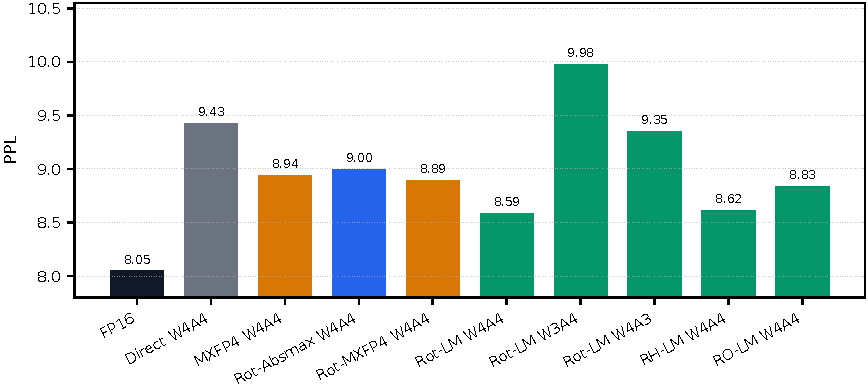
\includegraphics[width=0.88\linewidth]{image/stage_b_ppl.pdf}
  \caption{B 线 FFN-only model-level PPL 对比}
  \label{fig:stage-b-ppl}
\end{figure}

综上，B 线得到三点发现。第一，MXFP4 W4A4 是 FFN 中必须保留的强 baseline。第二，Rot-LM W4A4 在 local output 和 FFN-only PPL 上均优于 MXFP4 与 Rot-MXFP4。第三，Rot-LM W3A4 与 W4A3 仍具备可运行性，但其优势应表述为低比特可行性，而不是已经接近最强 W4A4 baseline。

\subsection{C 线：Attention/KV Cache 量化}

C 线实验回答的问题是：post-RoPE KV cache 的低比特量化是否能够保持 attention score 与 attention output，QJL residual 是否能进一步修正 Key quantization 的 inner-product 误差，以及 Attention 线性 W/A fake quant 与 KV cache low-bit quant 串联后，model-level PPL 是否仍可接受。实验依次考察 KV-local、QJL residual 和结构适配后的完整 Attention 层。

实验首先验证 post-RoPE Q/K 的 head-wise H64 rotation 在 no-quant 情形下保持 attention 计算不变性。随后，C2/C3 主要观察 score relative MSE、softmax KL、top-k overlap 和 output cosine；C4/C5 则采用 Attention 结构适配路径，将 Attention 线性层 W/A fake quant 与 KV cache 量化串联起来，分别评价整层输出误差与 Attention-only PPL。

表~\ref{tab:stage-c-kv-local} 汇总 C1 invariance 与 C2 KV-local 的关键结果。No-quant H64 rotation 的 score relative MSE 为 0，output cosine 为 1.0000，说明 post-RoPE Q/K 的 head-wise rotation 本身不破坏 attention score。进入 KV quantization 后，Hadamard-LM K4V4 明显优于 Absmax K4V4；Hadamard-LM K3V4 仍具备局部可行性，但误差明显高于 K4V4。head-internal H32 与 head-wise H64 的结果非常接近，说明 TinyLlama 的 64 维 head 内还存在更细 block rotation 的可行空间。

\begin{table}[!htbp]
  \centering
  \caption{C 线 C1/C2 attention-local 指标汇总}
  \label{tab:stage-c-kv-local}
  \footnotesize
  \begin{tabular}{llrrrr}
    \toprule
    Method & KV Bits & Score MSE & Softmax KL & Top-k & Output Cosine \\
    \midrule
    H64 No-quant & K16V16 & 0.0000 & 0.0000 & 1.0000 & 1.0000 \\
    Absmax & K4V4 & 0.0155 & 0.0464 & 0.8477 & 0.9448 \\
    Hadamard-LM H64 & K4V4 & 0.0035 & 0.0095 & 0.9189 & 0.9868 \\
    Hadamard-LM H32 & K4V4 & 0.0034 & 0.0090 & 0.9214 & 0.9868 \\
    Hadamard-LM H64 & K3V4 & 0.0132 & 0.0353 & 0.8568 & 0.9589 \\
    Hadamard-LM H32 & K3V4 & 0.0130 & 0.0339 & 0.8605 & 0.9593 \\
    Hadamard-LM H64 & K2V4 & 0.0421 & 0.5654 & 0.5343 & 0.9272 \\
    \bottomrule
  \end{tabular}
\end{table}

\begin{figure}[!htbp]
  \centering
  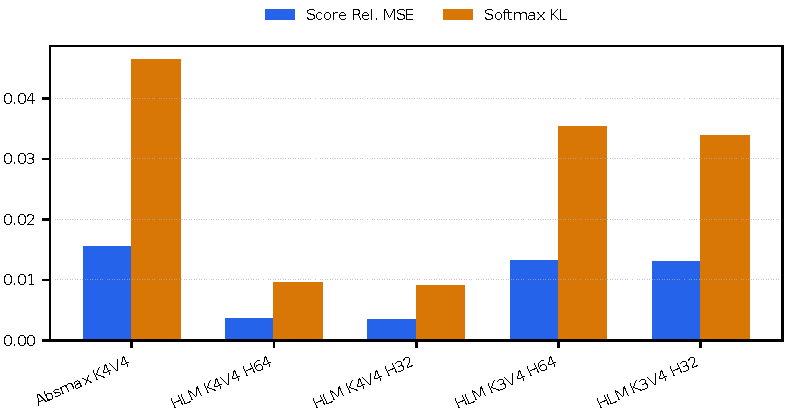
\includegraphics[width=0.88\linewidth]{image/stage_c_kv_local.pdf}
  \caption{C 线 KV-local score relative MSE 与 softmax KL 对比}
  \label{fig:stage-c-kv-local}
\end{figure}

表~\ref{tab:stage-c-qjl} 给出 QJL residual 结果。QJL correction 确实降低了部分 inner-product bias，例如 K3 base 的 bias 从 1.0115 降至 0.2042；但是 score relative MSE、softmax KL、top-k overlap 和 output cosine 均变差。K2 base 上也出现同样趋势。因此，当前 QJL residual 不进入 C5 默认实验组。

\begin{table}[!htbp]
  \centering
  \caption{C 线 C3 QJL residual 对比}
  \label{tab:stage-c-qjl}
  \footnotesize
  \begin{tabular}{lrrrr}
    \toprule
    Method & Score MSE & Softmax KL & Top-k & Output Cosine \\
    \midrule
    Hadamard-LM K2 & 0.0421 & 0.5654 & 0.5343 & 0.9272 \\
    Hadamard-LM K2 + QJL & 0.0595 & 0.9660 & 0.4917 & 0.8891 \\
    Hadamard-LM K3 & 0.0116 & 0.1834 & 0.6902 & 0.9764 \\
    Hadamard-LM K3 + QJL & 0.0176 & 0.2974 & 0.6452 & 0.9605 \\
    \bottomrule
  \end{tabular}
\end{table}

表~\ref{tab:stage-c-attention-local} 汇总结构适配后的 Attention-layer local 结果。Identity wrapper 的 layer output relative MSE 接近 0，说明 wrapper 本身不引入可见误差。KV-only K4V4 的 layer output cosine 为 0.9880；加入 Attention 线性 W/A fake quant 后，Rot-LM W4A4 + HLM K4V4 的 cosine 为 0.9569，优于 MXFP4 与 Rot-MXFP4 对照。Rot-LM W3A4 + HLM K3V4 的误差显著增大，表明 Attention 结构对 weight/key 同时降位宽更敏感。

\begin{table}[!htbp]
  \centering
  \caption{C 线 C4 structured Attention local output 汇总}
  \label{tab:stage-c-attention-local}
  \footnotesize
  \begin{tabular}{lllrr}
    \toprule
    Method & Linear Bits & KV Bits & Relative MSE & Cosine \\
    \midrule
    Attn Identity FP16 & FP16 & K16V16 & 0.0000 & 1.0000 \\
    Attn KV-HLM K4V4 & FP16 & K4V4 & 0.0246 & 0.9880 \\
    Attn MXFP4 + HLM K4V4 & W4A4 & K4V4 & 0.1200 & 0.9425 \\
    Attn Rot-MXFP4 + HLM K4V4 & W4A4 & K4V4 & 0.1223 & 0.9413 \\
    Attn Rot-LM W4A4 + HLM K4V4 & W4A4 & K4V4 & 0.0891 & 0.9569 \\
    Attn Rot-LM W3A4 + HLM K3V4 & W3A4 & K3V4 & 0.2558 & 0.8817 \\
    \bottomrule
  \end{tabular}
\end{table}

图~\ref{fig:stage-c-ppl} 给出 Attention-only model-level PPL。KV-only K4V4 H64 与 H32 的 PPL 分别为 8.20 和 8.21，均接近 FP16。加入 Attention 线性 W/A fake quant 后，MXFP4 W4A4 + HLM K4V4、Rot-MXFP4 W4A4 + HLM K4V4 与 Rot-LM W4A4 + HLM K4V4 的 PPL 分别为 9.00、8.93 和 8.61。Rot-LM W3A4 + HLM K3V4 升至 11.36，说明进一步降 weight/key 位宽会带来明显累积误差。

\begin{figure}[!htbp]
  \centering
  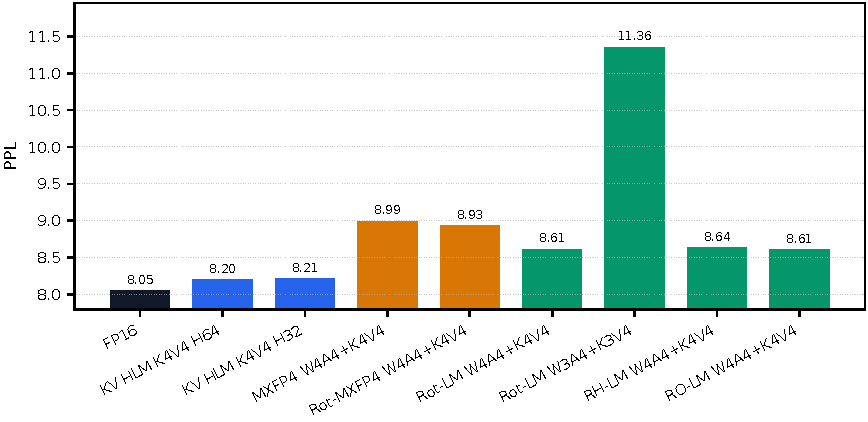
\includegraphics[width=0.90\linewidth]{image/stage_c_ppl.pdf}
  \caption{C 线 Attention-only model-level PPL 对比}
  \label{fig:stage-c-ppl}
\end{figure}

综上，C 线得到四点发现。第一，post-RoPE Q/K head-wise H64 rotation 在 no-quant 下保持 attention score 和 output，H32 也是可行的 head 内结构选项。第二，Hadamard-LM K3V4 在 KV-local 指标上可运行，但 K4V4 更稳定，K2V4 是失败边界。第三，当前 QJL residual 虽降低部分 inner-product bias，但整体 attention 指标变差，不适合作为默认方法。第四，Attention 结构适配后，Rot-LM W4A4 + HLM K4V4 的 PPL 接近 FP16；W3A4 + K3V4 仍可运行但退化明显，C 线低 bit 敏感性高于 FFN。

\section{实验结论}

当前实验的核心结论是：Hadamard rotation 与 Lloyd-Max codebook 在 TinyLlama 上能够显著改善低比特 fake quant 的数值质量，但其收益主要体现为数值误差下降和位宽边界探索，而不是直接的系统加速。

A 线表明，MXFP4 W4 已是强 baseline，Hadamard-LM W4 在 tensor reconstruction 和 PPL 上仍保持最稳定的数值质量。Hadamard-LM W3 可运行，但相对 W4 baseline 存在明确 PPL gap；W2 虽有较好的 tensor reconstruction 指标，但 PPL 已经崩溃，暂时应视为失败边界。

B 线表明，FFN 中的 W/A fake quant 与 local output 指标具有较好一致性。MXFP4 W4A4 是必须保留的强 baseline，而 Rot-LM W4A4 在 local output 和 FFN-only PPL 上均更优。Rot-LM W3A4 和 Rot-LM W4A3 仍具备可运行性，但相对强 W4A4 baseline 的差距需要在结论中保留。

C 线表明，Attention/KV cache 对结构适配更敏感。post-RoPE Q/K head-wise H64 rotation 在 no-quant 下保持计算不变性，H32 与 H64 在 KV-local 和 KV-only PPL 上接近；Hadamard-LM K3V4 在 KV-local 层面可行，K2V4 是失败边界；当前 QJL residual 未能改善整体 attention 指标。经过 Attention 结构适配后，KV-only K4V4 和 structured W4A4 + K4V4 的 PPL 接近 FP16，但 W3A4 + K3V4 的误差仍明显更大。

补充实验进一步给出三点修正。第一，MXFP4 是更现实的 FP4 baseline，不能只与 uniform absmax 比较。第二，Lloyd-Max 在旋转域中的数值误差整体优于 MXFP4，但它不是标准 INT/FP GEMM 友好的格式，需要未来的 codebook-aware compute 支持。第三，rotation block size 会影响低 bit 结果，32/64 在 W3 或 W3A4 组上通常比 128 更稳，后续评价 3-bit 可行性时应将 block size 作为正式超参数。

因此，当前实验最可靠的发现是：Hadamard rotation 负责削弱 outlier 并重塑分布，Lloyd-Max codebook 在旋转域中进一步降低低比特量化误差；二者结合能够在 weight-only、FFN W/A 和 KV-local 场景中给出低比特可行性的算法证据。后续工作应集中在两点：一是将这些 fake quant 结果转化为可实现的 bit packing、codebook lookup 或专用 kernel；二是继续改进 Attention 结构量化，尤其是更稳健的 Key 低比特表示和 residual correction 方法。

\printbibliography[heading=bibintoc, title=\ebibname]

\end{document}
